\documentclass[11pt]{article}
\title{\textbf{Meccano fox-surd frame}}
\author{https://github.com/heptagons/meccano/frames/fox-surd}
\date{}

\usepackage{../../meccano}
\usepackage{tikz}
\usetikzlibrary{calc}

\begin{document}

\maketitle
\begin{abstract}
Meccano\meccanoref fox-surd frame is a generalization of fox-frame\footnote{
\href{https://github.com/heptagons/meccano/blob/main/frames/fox/fox.pdf}{Meccano fox frame }}
where at least one of the frame's strips size is no longer an integer but a surd.
\end{abstract}

\section{Pentagons fox-surd}

\begin{figure}[H]
\centering
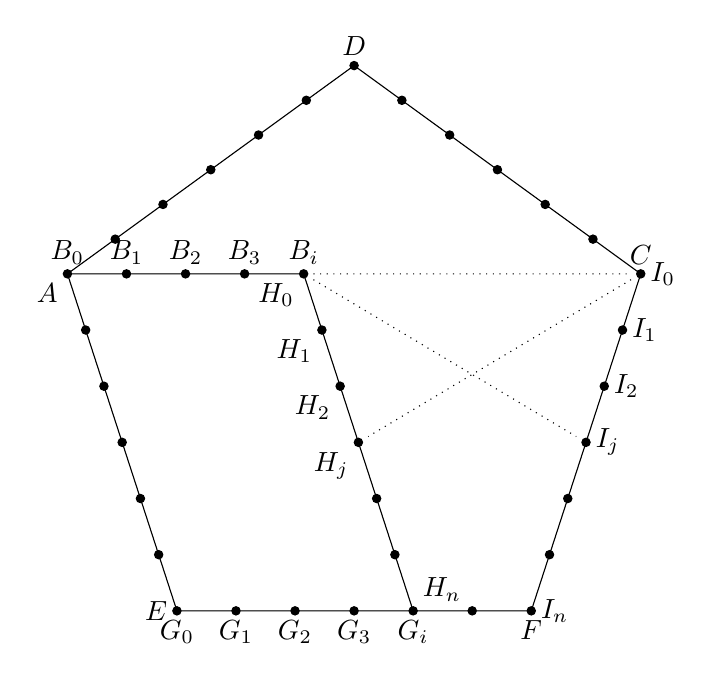
\begin{tikzpicture}
\begin{scope}[scale=0.75]
\begin{scope}
\draw[fill=black] (0,0) circle(2pt) node[above]{$B_0$}
-- ++(1,0) circle(2pt) node[above]{$B_1$}
-- ++(1,0) circle(2pt) node[above]{$B_2$}
-- ++(1,0) circle(2pt) node[above]{$B_3$}
-- ++(1,0) circle(2pt) node[above]{$B_i$} node[below left]{$H_0$} node(bi){}
-- ++(-72:1) circle(2pt) node[below left]{$H_1$}
-- ++(-72:1) circle(2pt) node[below left]{$H_2$}
-- ++(-72:1) circle(2pt) node[below left]{$H_j$} node(hj){}
-- ++(-72:1) circle(2pt)
-- ++(-72:1) circle(2pt)
-- ++(-72:1) circle(2pt) node[above right]{$H_n$} node[below]{$G_i$}
-- ++(-1,0) circle(2pt) node[below]{$G_3$}
-- ++(-1,0) circle(2pt) node[below]{$G_2$}
-- ++(-1,0) circle(2pt) node[below]{$G_1$}
-- ++(-1,0) circle(2pt) node[below]{$G_0$} node[left]{$E$}
-- ++(108:1) circle(2pt)
-- ++(108:1) circle(2pt)
-- ++(108:1) circle(2pt)
-- ++(108:1) circle(2pt)
-- ++(108:1) circle(2pt)
-- ++(108:1);
\draw[fill=black] (0,0) node[below left]{$A$}
-- ++(36:1) circle(2pt)
-- ++(36:1) circle(2pt)
-- ++(36:1) circle(2pt)
-- ++(36:1) circle(2pt)
-- ++(36:1) circle(2pt)
-- ++(36:1) circle(2pt) node[above]{$D$}
-- ++(-36:1) circle(2pt)
-- ++(-36:1) circle(2pt)
-- ++(-36:1) circle(2pt)
-- ++(-36:1) circle(2pt)
-- ++(-36:1) circle(2pt)
-- ++(-36:1) circle(2pt) node[above]{$C$} node[right]{$I_0$} node(i0){}
-- ++(-108:1) circle(2pt) node[right]{$I_1$}
-- ++(-108:1) circle(2pt) node[right]{$I_2$}
-- ++(-108:1) circle(2pt) node[right]{$I_j$} node(ij){}
-- ++(-108:1) circle(2pt)
-- ++(-108:1) circle(2pt)
-- ++(-108:1) circle(2pt) node[below]{$F$} node[right]{$I_n$}
-- ++(-1,0) circle(2pt)
-- ++(-1,0);

\draw[dotted] (bi) -- (ij) (i0) -- (hj) (bi) -- (i0);

\end{scope}
\end{scope}
\end{tikzpicture}
\caption{Pentagon of size $n$ where each segment separated by circles represents a unit.
We have a surd frame formed by the six points: $B_i$, $I_0$, $H_j$, $I_j$, $H_n$ and $I_n$.
By iterating the values $i,j = 0,...,n$ we'll get diverse frames.
}

\label{fig:pentagon}
\end{figure}

From figure \ref{fig:pentagon} the fox-surd frame has three real strips of integer size:
\begin{itemize}
    \item $\overline{B_iG_i}$ of size $n$.
    \item $\overline{G_iI_n}$ of size $n-i$, where $i = 0,...,n$.
    \item $\overline{I_0I_n}$ of size $n$.
\end{itemize}
The other two strips are generic in the sense the sizes can be surds:
\begin{itemize}
	\item $\overline{B_iI_j}$ of size to be determined $f(n,i,j)$, where $i,j = 0,...,n$.
	\item $\overline{H_jI_0}$ of equal size of $\overline{B_iI_j}$.
\end{itemize}

From the regular pentagon we know the main diagonal $\overline{AC}$ equals
$\frac{1+\sqrt{5}}{2}n$ where $n$ is the pentagon side size. We can calculate different
segments of the main diagonal iterating $i = 0,...,n$:
\begin{align}
B_0 &\equiv A \nonumber\\
\overline{B_0C} &= \frac{1+\sqrt{5}}{2}n \\
\overline{B_iC} &= \frac{1+\sqrt{5}}{2}n - i \nonumber\\
 &= \frac{n-2i}{2} + \frac{n\sqrt{5}}{2}, \quad i = 0, ..., n \nonumber\\
 &= \frac{x_i}{2} + \frac{n\sqrt{5}}{2}, \quad x_i = n - 2i \label{eq:B_iC}
\end{align}

From the regular pentagon we know the angle ${B_iCI_j}$ equals $2\pi / 5$ so we have:
\begin{align}
\theta &\equiv \angle{B_iCI_j} \\
\cos\theta &= \cos\frac{2\pi}{5} = \frac{\sqrt{5}-1}{4} \label{eq:cosine}
\end{align}

\subsection{Pentagon surds sizes}

Using the law of cosines we can calculate one of the frame surds $s_{ij} \equiv \overline{B_iI_j}$.
We notice the value of $\overline{CI_j}$ equals $j$, and we'll use the values of $\overline{B_iC}$ from equation \ref{eq:B_iC}, and the cosine value from equation \ref{eq:cosine} to get:
\begin{align}
s_{ij}^2 &\equiv \overline{B_iI_j}^2 \\
 &= \overline{CI_j}^2 + \overline{B_iC}^2 
 - 2\overline{CI_j}\times\overline{B_iC}\cos\theta  \nonumber\\
 &= j^2 + \left(\frac{x_i}{2} + \frac{n\sqrt{5}}{2}\right)^2
 - 2j\left(\frac{x_i}{2} + \frac{n\sqrt{5}}{2}\right)\left(\frac{\sqrt{5} - 1}{4}\right) \\
 &= j^2 + \frac{1}{4}\left(x_i + n\sqrt{5}\right)^2
 - \frac{j}{4}\left(x_i + n\sqrt{5}\right)\left(\sqrt{5}-1\right)
\end{align}   

We multiply both sides by 4 and simplify:   
\begin{align}
(2s_{ij})^2 &= 4j^2 + (x_i + n\sqrt{5})^2 - j(x_i + n\sqrt{5})(\sqrt{5} - 1) \\
 &= 4j^2 + x_i^2 + 2x_in\sqrt{5} + 5n^2 - j(x_i\sqrt{5} - x_i + 5n - n\sqrt{5})\\
 &= 4j^2 + x_i^2 + 5n^2 + x_ij - 5nj + (2nx_i - x_ij + nj)\sqrt{5}
\end{align}
In order to have a simpler $(2s_i)^2 = u+v\sqrt{5}$ we define two variables $u$ and $v$.
We replace again $x_i = n - 4i$ defined in equation \ref{eq:B_iC}:
\begin{align}
u &\equiv 4j^2 + x_i^2 + 5n^2 + x_ij - 5nj \nonumber\\
 &= 4j^2 + (n-2i)^2 + 5n^2 + (n-2i)j - 5nj \nonumber\\
 &= 4j^2 + n^2 - 4ni + 4i^2 + 5n^2 + nj - 2ij - 5nj \nonumber\\
 &= 6n^2 + 4i^2 + 4j^2 - 4ni - 4nj - 2ij  \label{eq:u}\\
v &\equiv 2nx_i - x_ij + nj \nonumber\\
 &= 2n(n-2i) - (n-2i)j + nj \nonumber\\
 &= 2n^2 - 4ni - nj + 2ij + nj \nonumber\\
 &= 2n^2 - 4ni + 2ij \label{eq:v}\\
\end{align}
Finally we have $s_{ij}$ in function of $n,i,j$ the side:
\begin{align}
s_{ij} &= \frac{\sqrt{u+v\sqrt{5}}}{2} \nonumber\\
 &= \frac{\sqrt{6n^2 + 4i^2 + 4j^2 - 4ni - 4nj - 2ij + (2n^2 - 4ni + 2ij)\sqrt{5}}}{2}
\end{align}

\subsection{Pentagons surds simplification}

If value $v$ from equation \ref{eq:v} is zero $s_{ij}$ simplifies to $\sqrt{u}/2$:
\begin{align}
v &= 0 \nonumber\\
2n^2 - 4ni + 2ij &= 0 \nonumber\\
n^2 - 2ni + ij &= 0 \nonumber\\
\end{align}




\end{document}